%\documentclass[handout]{beamer} % Sin animaciones
% https://tex.stackexchange.com/questions/74805/latex-error-option-clash-for-package-xcolor
\documentclass[xcolor={dvipsnames},spanish]{beamer}
%\usetheme{Warsaw}
\usetheme{Madrid}
\setbeamertemplate{navigation symbols}{} % remove navigation symbols
%\setbeamercolor{alerted text}{fg=orange}

\usepackage{thesis}
\usepackage{sections/nd_rules}
\setbeamertemplate{footline}[frame number]

% https://tex.stackexchange.com/questions/464916/listing-inside-a-frame-using-beamer
\lstset{language=ppa, xleftmargin=0.5cm}

\usepackage{fitch}

% https://tex.stackexchange.com/questions/178800/creating-sections-each-with-title-pages-in-beamers-slides
\AtBeginSection[]{
  \begin{frame}
  \vfill
  \centering
  \begin{beamercolorbox}[sep=8pt,center,shadow=true,rounded=true]{title}
    \usebeamerfont{title}\insertsectionhead\par%
  \end{beamercolorbox}
  \vfill
  \end{frame}
}

\newenvironment{command}
    {
        \begin{beamercolorbox}[sep=8pt,center,shadow=true,rounded=true]{block body}
    }
    {\end{beamercolorbox}}

% Tiempo total para dar la presentación: 60 minutos, 15 para preguntas

% Notas

\title{PPA}
\subtitle{Un asistente de demostración para
lógica de primer orden con extracción de
testigos usando la traducción de Friedman}
\author{Manuel Panichelli}
\institute{Deparatamento de Computación, FCEyN, UBA}
\date{Diciembre 2024}

\begin{document}


\frame{\titlepage}

\section{Introducción}

% TODO: Considerar explicar que es un teorema y qué es la verificación
\begin{frame}{Asistentes de demostración}
    \begin{itemize}
        \item Los \textbf{asistentes de demostración} son herramientas que
        facilitan la escritura y el chequeo de demostraciones por
        computadora.
        \item Usos usuales: formalización de teoremas matemáticos y verificación de programas.
        \item Ventajas:\footnote{\href{https://youtu.be/AayZuuDDKP0?si=eGETzgh9PQ_8JecR}{Terrence Tao - Machine Assisted Proof}}
        \begin{itemize}
            \item Facilitan la colaboración a gran escala (mediante la confianza en el asistente).
            \item Habilitan generación automática de demostraciones con IA. Por ej. un \textit{LLM} (como \textit{ChatGPT}) suele devolver alucinaciones, que pueden ser filtradas automáticamente con un asistente.
        \end{itemize}
    \end{itemize}
\end{frame}

\begin{frame}{Asistentes de demostración}
    Implementan distintas \textit{teorías}. \todo{No me gusta teoria, se usa
    para teorias de primer orden}
    Ejemplos:
    \begin{itemize}
        \item Mizar (lógica de primer orden)
        \item Coq (teoría de tipos)
        \item Agda (teoría de tipos)
        \item Isabelle (lógica de orden superior / teoría de conjuntos ZF)
    \end{itemize}
\end{frame}

\begin{frame}{PPA}
    \begin{itemize}
        \item Diseñamos e implementamos \textbf{PPA} (\textit{Pani's Proof
        Assistant}), un asistente de demostración para lógica \textbf{clásica}
        de primer orden.
        \item Permite hacer extracción de testigos: dada una demostración de
        $\exists \var . \pred(\var)$, encuentra $\term$ tal que $\pred(\term)$.
        \item Aporte principal: implementación de extracción de testigos para lógica clásica de forma directa (vemos los detalles después).
    \end{itemize}
    
\end{frame}

\begin{frame}{Representación de demostraciones}
    Queremos escribir demostraciones en la computadora. ¿Cómo las representamos?. Veamos un ejemplo.
    
    \begin{itemize}
        \item Tenemos dos premisas
        \begin{enumerate}
            \item Los alumnos que faltan a los exámenes, los reprueban.
            \item Si se reprueba un final, se recursa la materia.
        \end{enumerate}
        \item A partir de ellas, podríamos demostrar que si un alumno falta a un final, entonces recursa la materia.
    \end{itemize}

    \begin{block}{Teorema}
        Si ((falta entonces reprueba) y (reprueba entonces recursa)) y falta, entonces recursa
    \end{block}
    \begin{exampleblock}{Demostración}
        \begin{itemize}
    \item Asumo que falta. Quiero ver que recursa.
    \item Sabemos que si falta, entonces reprueba. Por lo tanto reprobó.
    \item Sabemos que si reprueba, entonces recursa. Por lo tanto recursó. \qed
\end{itemize}
    \end{exampleblock}
\end{frame}

\begin{frame}{Sistemas deductivos}
    \begin{itemize}
        \item La demostración anterior es poco precisa. No se puede representar rigurosamente.
        \item Necesitamos \textbf{sistemas deductivos}: sistemas lógicos formales usados para demostrar setencias. Pueden ser representados como un tipo abstracto de datos.
        \item Usamos \textbf{deducción natural}. Compuesto por,
        \begin{itemize}
            \item \textbf{Lenguaje formal}: lógica de primer orden.
            \item \textbf{Reglas de inferencia}: lista de reglas que se usan para probar teoremas a partir de axiomas y otros teoremas. Por ejemplo, \textit{modus ponens} (si
    es cierto $\form \fImp \formTwo$ y $\form$, se puede concluir $\formTwo$) o
    \textit{modus tollens} (si es cierto $\form \fImp \formTwo$ y $\fNot
    \formTwo$, se puede concluir $\fNot\form$)
    \item \textbf{Axiomas}: fórmulas de $L$ que se asumen válidas. Todos los
    teoremas se derivan de axiomas. Se usan para modelar \textit{teorías} de
    primer orden (por ej. teoría de estudiantes en la facultad).
        \end{itemize}
    \end{itemize}
\end{frame}

\begin{frame}{Lógica de primer orden}

\begin{definition}[Términos]
    Los términos están dados por la gramática:
    \begin{align*}
        \term ::= &\ \var                               &\text{(variables)} \\
                  & \mid \fun(\term_1, \dots, \term_n) &\text{(funciones)}
    \end{align*}
\end{definition}
\begin{definition}[Fórmulas]
    Las fórmulas están dadas por la gramática:
    \begin{align*}
        \form, \formTwo ::=
         & \ \pred(\term_1, \dots, \term_n) & (\text{predicados})                \\
         & \mid \fFalse                     
           \mid \fTrue                      & \text{(falso o \textit{bottom} y verdadero o \textit{top})} \\
         & \mid \form \fAnd \formTwo                        
           \mid \form \fOr \formTwo           & \text{(conjunción y disyunción)}     \\
         & \mid \form \fImp \formTwo                       
           \mid \fNot \form                 & \text{(implicación y negación)}                  \\
         & \mid \forall \var . \form        
           \mid \exists \var . \form        & \text{(cuantificador universal y existencial)}
    \end{align*}
\end{definition}

\end{frame}

\begin{frame}{Lógica de primer orden}
Los predicados son \textbf{fórmulas atómicas}. Los de aridad 0 además son llamados \textit{variables proposicionales}.

\begin{notation*}
    Usamos
    \begin{itemize}
        \item $\var, \varTwo, \varThree, \dots$ como \textbf{variables}.
        \item $\fun, \funTwo, \funThree, \dots$ como \textbf{símbolos de función}.
        \item $\pred, \predTwo, \predThree, \dots$ como \textbf{símbolos de predicado}.
        \item $\term, \termTwo, \dots$ para referirnos a \textbf{términos}.
        \item $\formLit, \formLitTwo, \formLitThree, \dots$, $\form, \formTwo, \formThree, \dots$ y $\anyForm, \anyFormTwo, \dots$ para referirnos a \textbf{fórmulas}.
    \end{itemize}
\end{notation*}
\end{frame}

\section{Deducción natural}

\begin{frame}{Deducción natural}
    \begin{definitions}
        \begin{itemize}
            \item $\ctx$ es un \textbf{contexto de demostración}, conjunto de
            fórmulas que se asumen válidas
            \item Notación: $\ctx, \anyForm = \ctx \cup \{\anyForm\}$
            \item $\judG$ es la \textbf{relación de derivabilidad} definida a
            partir de las \textit{reglas de inferencia}. Permite escribir
            juicios $\ctx \judG \anyForm$.
            \item Intuición: \textit{``$\anyForm$ es
            una consecuencia de las suposiciones de $\ctx$''}
            \item El juicio es cierto si en una cantidad finita de
            pasos podemos concluir $\anyForm$ a partir de las fórmulas de
            $\ctx$, los axiomas y las reglas de inferencia.
            \item Decimos que
            $\anyForm$ es \textit{derivable} a partir de $\ctx$.
        \end{itemize}
    \end{definitions}
\end{frame}

\begin{frame}{Reglas de inferencia}
    \begin{definition}[Reglas de inferencia]
        \begin{columns}
            \column{0.5\textwidth}
            \proofTreeAx
            \proofTreeImpI
            \proofTreeImpE
            \column{0.5\textwidth}
            \proofTreeAndI
            \proofTreeAndEOne
            \proofTreeAndETwo
        \end{columns}
        
    \end{definition}
    Dos tipos para cada conectivo y cuantificador, dada una fórmula formada con un conectivo:
    \begin{itemize}
        \item \textbf{Introducción}: ¿Cómo la demuestro?
        \item \textbf{Eliminación}: ¿Cómo la uso para demostrar otra?
    \end{itemize}
\end{frame}

\begin{frame}{Ejemplo}
    Vamos a demostrar el ejemplo informal en deducción natural. Lo modelamos
    para un alumno y materia particulares. Notamos:
    \begin{itemize}
        \item $\reprueba \equiv \predReprueba(juan, \funFinal(logica))$
        \item $\recursa \equiv \predRecursa(juan, logica)$
        \item $\falta \equiv \predFalta(juan, \funFinal(logica))$
    \end{itemize}

    Queremos probar entonces 
    \[
        \Big(
            (\falta \fImp \reprueba) \wedge (\reprueba \fImp \recursa)
        \Big)
        \fImp
        (\falta \fImp \recursa)
    \]
\end{frame}

\begin{frame}{Ejemplo}
    \begin{prooftree}
        \AxiomC{}
        \RL{\ruleAx}
        \UnaryInfC{$\ctx \judG (\falta \fImp \reprueba) \wedge (\reprueba \fImp \recursa)$}
        \RL{\ruleAndEOne}
        \UnaryInfC{$\ctx \judG \reprueba \fImp \recursa$}
        
        \AxiomC{$\someProof$}
        \noLine
        \UnaryInfC{$\ctx \judG \reprueba$}
        \RL{\ruleImpE}
        \BinaryInfC{\(
            \ctx =
            (\falta \fImp \reprueba) \wedge (\reprueba \fImp \recursa),\
            \falta
            \judG
            \recursa
        \)}
        \RL{\ruleImpI}
        \UnaryInfC{\(
            (\falta \fImp \reprueba) \wedge (\reprueba \fImp \recursa)
            \judG
            \falta \fImp \recursa 
        \)}
        \RL{\ruleImpI}
        \UnaryInfC{\(
            \judG
            \Big(
                (\falta \fImp \reprueba) \wedge (\reprueba \fImp \recursa)
            \Big)
            \fImp
            (\falta \fImp \recursa)
        \)}
    \end{prooftree}

    donde

    \begin{prooftree}
        \AxiomC{}
        \RL{\ruleAx}
        \UnaryInfC{$\ctx \judG (\falta \fImp \reprueba) \wedge (\reprueba \fImp \recursa)$}
        \RL{\ruleAndETwo}
        \UnaryInfC{$\ctx \judG \falta \fImp \reprueba$}
        \AxiomC{}
        \RL{\ruleAx}
        \UnaryInfC{$\ctx \judG \falta$}
        \RL{\ruleImpE}
        \LL{$\someProof=$}
        \BinaryInfC{$\ctx \judG \reprueba$}
    \end{prooftree}
\end{frame}

\begin{frame}{Reglas de inferencia}
    \begin{definition}[Reglas de inferencia]
        \proofTreeLEM
        \begin{columns}
            \begin{column}{0.5\textwidth}
                \proofTreeFalseE
                \proofTreeTrueI
            \end{column}
            \begin{column}{0.5\textwidth}
                \proofTreeNotI
                \proofTreeNotE
            \end{column}
        \end{columns}
        \begin{columns}
            \begin{column}{0.5\textwidth}
                \proofTreeOrIOne
            \end{column}
            \begin{column}{0.5\textwidth}
                \proofTreeOrITwo
            \end{column}
        \end{columns}
        \proofTreeOrE
    \end{definition}
\end{frame}

\begin{frame}{Reglas de inferencia}
    \begin{definition}[Sustitución]
        Notamos como $\form \subst{\var}{\term}$ a la sustitución de todas las
        ocurrencias libres de la variable $\var$ por el término $\term$ en la
        fórmula $\form$.
    \end{definition}
    \begin{definition}[Reglas de cuantificadores]
        \begin{columns}
            \column{0.5\textwidth}
            \proofTreeForallI
            \column{0.5\textwidth}
            \proofTreeForallE
        \end{columns}
        \proofTreeExistsI
        \proofTreeExistsE
    \end{definition}
\end{frame}

\begin{frame}{Reglas admisibles}
    \begin{itemize}
        \item Mencionamos \textit{modus tollens} pero no aparece en las reglas de inferencia.
        \item Queremos un sistema lógico \textbf{minimal}: no agregamos como
        regla de inferencia lo que podemos derivar a partir de las existentes,
        las reglas \textbf{admisibles}.
        \item Se implementan como \textit{macros}: cada uso de la regla
        admisible se reemplaza por su demostración.
    \end{itemize} 

    \begin{lemma}[Modus tollens]
        
    \begin{prooftree}
        \AxiomC{}
        \RL{\ruleAx}
        \UnaryInfC{\(\ctx \judG (\form \fImp \formTwo) \fAnd \fNot \formTwo\)}
        \RL{\ruleAndETwo}
        \UnaryInfC{\(
            \ctx \judG \fNot \formTwo
        \)}
        \AxiomC{}
        \RL{\ruleAx}
        \UnaryInfC{\(\ctx \judG (\form \fImp \formTwo) \fAnd \fNot \formTwo\)}
        \RL{\ruleAndEOne}
        \UnaryInfC{$\ctx \judG \form \fImp \formTwo$}
        \AxiomC{}
        \RL{\ruleAx}
        \UnaryInfC{$\ctx \judG \form$}
        \RL{\ruleImpE}
        \BinaryInfC{\(
            \ctx \judG \formTwo
        \)}
        \RL{\ruleNotE{}}
        \BinaryInfC{\(
            \ctx = (\form \fImp \formTwo) \fAnd \fNot \formTwo, \form
            \judG
            \fFalse
        \)}
        \RL{\ruleNotI{}}
        \UnaryInfC{\(
            (\form \fImp \formTwo) \fAnd \fNot \formTwo
            \judG
            \fNot \form
        \)}
        \RL{\ruleImpI{}}
        \UnaryInfC{\(\judG
            (\form \fImp \formTwo \fAnd \fNot \formTwo)
            \fImp \fNot\form
        \)}
    \end{prooftree}
    \end{lemma}
\end{frame}

\begin{frame}{Sustitución sin capturas}
    Para la sustitución $\form \subst{\var}{\term}$ queremos evitar la
    \textbf{captura de variables}, por ejemplo
    \[
        (\forall \varTwo . \pred(\var))\subst{\var}{\varTwo} \overset{?}{=}
        \forall \varTwo . \pred(\alert{\varTwo})
    \]
    sustituyendo sin más, capturamos a la variable $\var$ que ahora está ligada.
    Lo evitamos \textbf{automáticamente}: cuando se encuentra con una captura,
    se renombra la variable ligada de forma que no ocurra
    \[
        (\forall \varTwo . \pred(\var))\subst{\var}{\varTwo} =
        \forall \alert{\varThree} . \pred(\varTwo)
    \]
\end{frame}

\begin{frame}{Alfa equivalencia}
    \begin{itemize}    
        \item Si tenemos una hipótesis $\exists \var . \pred(\var)$ queremos poder
        usarla para demostrar $\exists \varTwo . \pred(\varTwo)$.
        \item No son iguales, pero son \textbf{\bm{$\alpha$}-equivalentes}: si
        renombramos variables ligadas de forma apropiada, son iguales.
        \item Algoritmo naíf: cuadrático en la estructura de la fórmula,
        renombrando recursivamente.
        \item Algoritmo cuasilineal: manteniendo dos sustituciones, una por
        fórmula.
    \end{itemize}
    \begin{example}
        \begin{align*}
            (\exists \var . \fun(\var)) &\alphaEq (\exists \varTwo . \fun(\varTwo))
            &&\{\}, \{\}
            \\
            &\iff \fun(\var) \alphaEq \fun(\varTwo)
                &&\{\var \mapsto \varThree\}, \{\varTwo \mapsto \varThree\}\\
            &\iff \var \alphaEq \varTwo
                &&\{\var \mapsto \varThree\}, \{\varTwo \mapsto \varThree\}\\
            &\iff \varThree = \varThree.
        \end{align*}        
    \end{example}
\end{frame}

\section{PPA}

\begin{frame}{Mathematical vernacular}
    Aparentemente hay una forma canónica de presentar demostraciones matemáticas\footnote{\textit{Mathematical
    Vernacular} de Freek Wiedijk}. Descubierta e implementada independientemente en Mizar,
    Isar (Isabelle), etc. Combinación de ideas:

    \begin{itemize}
        \item \textbf{Deducción natural en estilo de \textit{Fitch}}. Notación
        equivalente en la cual las demostraciones son
        representadas como listas de fórmulas en lugar de árboles. Las que
        aparecen antes justifican las que aparecen después.
        \item \textbf{Reglas de inferencia \textit{``big step''}}: una forma de afirmar
        que $\form_1, \dots, \form_n \judG \form$ es válida, sin
        tener que demostrarlo a mano.
        \item \textbf{Sintaxis similar a un lenguaje de programación} en lugar del
        lenguaje natural usado para demostraciones.
    \end{itemize}
\end{frame}


% \begin{frame}{Deducción natural en estilo de Fitch}
%     En vez de árboles,
%     las demostraciones son listas de fórmulas, con las anteriores
%     justificando las posteriores.
%     \todo{Considerar dar un ejemplo para clarificar}
% \end{frame}

\begin{frame}[fragile]{PPA}
    Diseñamos e implementamos el \textit{lenguaje} PPA, inspirado en el
    \textit{mathematical vernacular}. Ejemplo:
    \lstinputlisting{listings/ppt/alumnos-corto.ppa}
\end{frame}

\begin{frame}[fragile]{Programas}
    Un \textbf{programa} de PPA consiste en una lista de \textbf{declaraciones},
    que pueden ser
    \begin{itemize}
        \item \textbf{Axiomas}: fórmulas que se asumen válidas
        \begin{lstlisting}[numbers=none]
axiom <name> : <form>
        \end{lstlisting}
        \item \textbf{Teoremas}: fórmulas junto con sus demostraciones.
\begin{lstlisting}[numbers=none]
theorem <name> : <form>
proof
    <steps>
end
\end{lstlisting}
    \end{itemize}
\end{frame}

\begin{frame}[fragile]{Identificadores}
    \begin{itemize}
        \item \textbf{Variables} (\lstinline{<var>})
        \begin{center}
            \verb/(\_|[A-Z])[a-zA-Z0-9\_\-]*(\')*/
        \end{center}
        \item \textbf{Identificadores} (\lstinline{<id>})
        \begin{center}
            \verb/[a-zA-Z0-9\_\-\?!#\$\%\*\+\<\>\=\?\@\^]+(\')*/
        \end{center}
        \item \textbf{Nombres} (\lstinline{<name>}) 
        \begin{center}
            \verb/\"[^\"]*\"/
        \end{center}
    \end{itemize}
\end{frame}

\begin{frame}[fragile]{Fórmulas y términos}
    Términos:
    \begin{itemize}
        \item Variables: \lstinline{<var>}
        \item Funciones: \lstinline{<id>(<term>, ..., <term>)}
    \end{itemize}

    Funciones:
    \begin{itemize}
        \item Predicados: \lstinline{<id>(<term>, ..., <term>)}
        \item \lstinline{<form> & <form>}
        \item \lstinline{<form> | <form>}
        \item \lstinline{<form> -> <form>}
        \item \lstinline{<form> <-> <form>}
        \item \lstinline{~ <form>}
        \item \lstinline{exists <var> . <form>}
        \item \lstinline{forall <var> . <form>}
        \item \lstinline{true}, \lstinline{false}
        \item \lstinline{(<form>)}
    \end{itemize}
\end{frame}

\begin{frame}{Demostraciones}
    \begin{itemize}
        \item Lista de comandos que reducen sucesivamente la \textit{tesis}
        (fórmula a demostrar) hasta agotarla por completo.
        \item Corresponden aproximadamente a reglas de inferencia de deducción
        natural (vistas como una demostración en el estilo de Fitch).
        \item Tienen disponible un \textbf{contexto} con todas las hipótesis
        asumidas (como axiomas) o demostradas (teoremas y comandos que
        demuestran hipótesis auxiliares).
    \end{itemize}
\end{frame}

\begin{frame}{by - El mecanismo principal de demostración}
    \begin{itemize}
        \item \lstinline{<form> by <name>, ..., <name>} afirma que la fórmula es una consecuencia lógica de las fórmulas que corresponden a las hipótesis provistas.
        \item Por debajo usa un \textit{solver} completo para lógica proposicional pero heurístico para primer órden.
        \item Se usa para eliminar implicaciones y universales.
        \item Usado por dos comandos principales: \lstinline{thus} y \lstinline{have}.
    \end{itemize}
\end{frame}


\begin{frame}[fragile]{Thus}
    \begin{command}
    \lstinline{thus <form> by <name>, ..., <name>}
    \end{command}

    Si \lstinline{<form>} es \textit{parte} de la tesis, y el \textit{solver} puede demostrar la implicación, lo demuestra automáticamente y lo descarga de la tesis.
    \begin{columns}
        \begin{column}{0.5\textwidth}
            \lstinputlisting{listings/interfaz/by-imp.ppa}
        \end{column}
        \begin{column}{0.5\textwidth}
            \lstinputlisting{listings/interfaz/by-forall.ppa}
        \end{column}
    \end{columns}
\end{frame}

\section{Certificador}

\begin{frame}{Certificados}
    \begin{itemize}
        \item Las demostraciones de \ppaLang se \textit{certifican} generando
        una demostración de deducción natural.
        \item Cumple con el criterio de de bruijn 
    \end{itemize}
    
\end{frame}

\section{Extracción de testigos}

% TODO: Considerar agregar ejemplo, pero seguro no alcanza el tiempo

% Acá arranca lo viejo

\begin{frame}{Introducción}
    \begin{itemize}
        \item PPA (\textit{Pani's proof assistant}) es un \textbf{asistente de demostraciones} inspirado en Mizar.
        \item Es un \textbf{lenguaje de programación} implementado en Haskell que permite escribir y chequear demostraciones en lógica \textit{clásica} de primer órden.
        \item A diferencia de Prolog, \textbf{no demuestra todo automáticamente}*. Deben ser escritas \textit{rigurosamente} por el usuario.
        \item (WIP) permite la extracción de testigos mediante la \textbf{traducción de Friedman}.
    \end{itemize}
\end{frame}

\begin{frame}{Asistentes de demostraciones (\textit{proof assistants})}
    \begin{itemize}
        \item Son programas que \textit{asisten} al usuario a la hora de escribir demostraciones, permiten representarlas en un programa
        \item Aplicaciones: Formalización de teoremas, verificación formal de programas, etc.
        \item Ejemplos: Coq, Isabelle (Isar), \textbf{Mizar}, $\dots$
        \item Ventajas\footnote{\href{https://youtu.be/AayZuuDDKP0?si=eGETzgh9PQ_8JecR}{Terrence Tao - Machine Assisted Proof}}:
        \begin{itemize}
            \item facilitan colaboración a gran escala (via confianza en el checker)
            \item habilitan generación automática de demostraciones con ML. Un LLM suele devolver alucinaciones, pero pueden ser chequeadas
        \end{itemize}
        
    \end{itemize}
\end{frame}

% TODO: Considerar mover para adelante

% TODO: usar referencias bien

\begin{frame}{Arquitectura de PPA}

\begin{figure}
    \centering
    %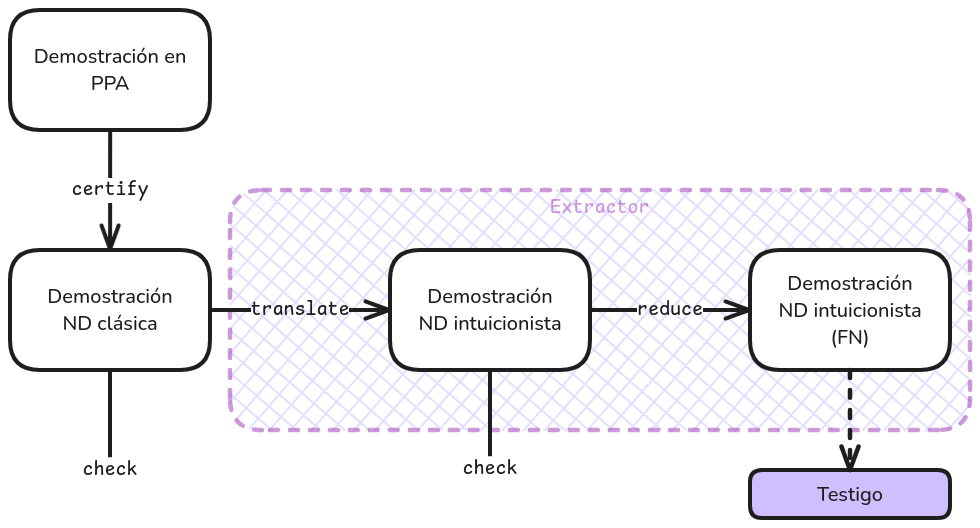
\includegraphics[width=1\linewidth]{arch.png}
\end{figure}

\end{frame}

\begin{frame}{¿Por qué certificados?}

    \begin{itemize}
        \item Si formalizamos una demostración en PPA y queremos chequear que sea correcta, hay que confiar en la implementación del \textit{proof assistant}.
        \item \textbf{Criterio de De Brujin}: si guardamos una demostración de bajo nivel de forma completa, puede ser chequeada por un programa independiente (que es sencillo de implementar).
        \item Cumplida por Coq, pero no Mizar\footnote{\href{https://www.researchgate.net/publication/225341870_A_Brief_Overview_of_Mizar}{Adam Naumowicz - A brief overview of Mizar}}.
    \end{itemize}

\end{frame}

\begin{frame}{PPA}
    \begin{itemize}
        \item Es un lenguaje. Frontend implementado con un \textit{parser generator} (happy + alex)
        \item Permite definir axiomas y teoremas con sus demostraciones, que al \textbf{certificarse} generan una demostración en deducción natural.
        \item Basado en \textit{Mathematical Vernacular}\footnote{\href{https://www.cs.ru.nl/~freek/notes/mv.pdf}{The Mathematical Vernacular - Freek Wiedijk}}: un leguaje formal para escribir demostraciones similar al natural.
    \end{itemize}
\end{frame}


\begin{frame}[fragile]{Ejemplo}
    Una demostración es una secuencia de \textit{comandos}, que pueden ir sucesivamente reduciendo la \textit{tesis} (objetivo a probar) y agregando hipótesis a un contexto. Se mapean a reglas de deducción natural.

\begin{block}{Teorema}
    \begin{Verbatim}[commandchars=\\\{\}]
\textbf{theorem} "implication transitivity":
    (a -> b) & (b -> c) -> (a -> c) // Tesis
\textbf{proof}        
    \textbf{suppose} h1: (a -> b) & (b -> c)
    // Tesis: a -> c
    
    \textbf{suppose} h2: a
    // Tesis: c
    
    \textbf{thus} c \textbf{by} h1, h2
\textbf{end}
\end{Verbatim}

\end{block}
\end{frame}

\begin{frame}{by}
    \begin{itemize}
        \item El mecanismo principal para demostrar es el \textbf{by}, que \textit{automáticamente} demuestra que un hecho es consecuencia de una lista de hipótesis.
        \item Se usa en lugar de \ruleE{$\to$} y \ruleE{$\forall$}
        \item Es completo para lógica proposicional pero heurístico para LPO
    \end{itemize}
\end{frame}

\begin{frame}[fragile]{Ejemplo}
\begin{block}{}
\begin{Verbatim}[commandchars=\\\{\}]
\textbf{axoim} ax1: a -> b
\textbf{axiom} ax2: a
\textbf{theorem} thm: b
\textbf{proof}
    \textbf{thus} b \textbf{by} ax1, ax2
\textbf{end}
\end{Verbatim}    
\end{block}

Para demostrar $\big( (a \to b) \wedge a \big) \to b$ lo hacemos por el absurdo: negamos y encontramos una contradicción.
\end{frame}

\begin{frame}[fragile]{DNF}
Primero convertimos la fórmula a forma normal disyuntiva (DNF)

\newcommand{\just}[1]{\textcolor{violet}{(#1)}}

\begin{align*}
    &\neg [ \big( (a \to b) \wedge a \big) \to b ] \\
    &\equiv \neg [ \neg \big( (a \to b) \wedge a \big) \vee b ]
        && \just{x \to y \equiv \neg x \vee y}\\
    &\equiv \neg \neg \big( (a \to b) \wedge a \big) \wedge \neg b
        && \just{\neg(x \vee y) \equiv \neg x \wedge \neg y}\\
    &\equiv \big( (a \to b) \wedge a \big) \wedge \neg b
        && \just{\neg\neg x \equiv x}\\
    &\equiv (\neg a \vee b) \wedge a \wedge \neg b
         && \just{x \to y \equiv \neg x \vee y}\\
    &\equiv (\neg a \vee b) \wedge a \wedge \neg b
        && \just{(x \vee y) \wedge z \equiv (x \wedge z) \vee (y \wedge z) }\\
    &\equiv
        (\neg a \wedge a \wedge \neg b)
        \vee
        (b \wedge a \wedge \neg b)
\end{align*}
\end{frame}

\begin{frame}{Contradicción}
    Ya tenemos la fórmula en DNF, ahora tenemos que demostrar la contradicción. Lo hacemos refutando cada cláusula
    \[
    (\alert{\neg a} \wedge \alert{a} \wedge \neg b)
        \vee
        (\alert{b} \wedge a \wedge \alert{\neg b}) \vdash \bot
    \]

    \begin{block}{Reglas}
        \begin{prooftree}
            \AxiomC{$\judg{\ctx}{\form \vee \formTwo}$}
            \AxiomC{$\judg{\ctx, \form}{\formThree}$}
            \AxiomC{$\judg{\ctx, \formTwo}{\formThree}$}
            \RL{\ruleE{$\vee$}}
            \TrinaryInfC{$\judg{\ctx}{\formThree}$}
        \end{prooftree}

        \begin{prooftree}
        \AxiomC{$\judg{\ctx}{\neg \form}$}
        \AxiomC{$\judg{\ctx}{\form}$}
        \RL{\ruleE{$\neg$}}
        \BinaryInfC{$\judg{\ctx}{\bot}$}
    \end{prooftree}
    \end{block}
\end{frame}

\begin{frame}{Recap by}
    Teniendo en el contexto $\Gamma = \{ h_1 : b_1, \dotso, h_n : b_n\}$
    para certificar
    $$\text{thus } a \text{ by } h_1 \dots h_n$$

    \begin{itemize}
        \item Debe demostrar $b_1 \wedge \dotso \wedge b_n \to a$
        \item Lo hace por absurdo: la niega y encuentra una contradicción
        \item Primero la convierte a forma normal disyuntiva (DNF)
        \item Luego refuta cada cláusula (conjunción de literales)
        \begin{itemize}
            \item False ($\bot \wedge p \wedge q$)
            \item Literales opuestos ($p(a) \wedge \neg p(a) \wedge q$)
            \item Eliminación de existencial ($\forall x. p(x) \wedge \neg p(a))$
        \end{itemize}
    \end{itemize}

    \begin{alertblock}{}
    \textbf{Desafío}: ¡Hay que generar una demostración de deducción natural!
    \end{alertblock}
\end{frame}

\begin{frame}{DNF}
    ¿Cómo demostramos el pasaje de uno al otro?
    \begin{gather*}
        \neg [ \big( (a \to b) \wedge a \big) \to b ] \vdash \bot\\
        \vdots\\
        (\neg a \wedge a \wedge \neg b) \vee (b \wedge a \wedge \neg b) \vdash \bot
    \end{gather*}

    Generando demostraciones para todas las equivalencias, y convirtiendo la fórmula paso por paso (\textit{``small step''})
    \begin{columns}
        \column{0.5\textwidth}
        \begin{align*}
        \neg\neg x &\equiv x\\
        \neg \bot &\equiv \top\\
        \neg \top &\equiv \bot\\
        x \to y &\equiv \neg x \vee y\\
        \neg(x \vee y) &\equiv \neg x \wedge \neg y\\
        \neg(x \wedge y) &\equiv \neg x \vee \neg y
    \end{align*}
        \column{0.5\textwidth}
        \begin{align*}
            (x \vee y) \wedge z &\equiv (x \wedge z) \vee (y \wedge z)\\
            z \wedge (x \vee y) &\equiv (z \wedge x) \vee (z \wedge y)\\
            x \vee (y \vee z) &\equiv (x \vee y) \vee z\\
            x \wedge (y \wedge z) &\equiv (x \wedge y) \wedge z
        \end{align*}
    \end{columns}
\end{frame}

\begin{frame}{DNF}
    Para poder hacerlo paso por paso también hace falta demostrar la \textit{congruencia} de los operadores

    \[
        a \vee \alert{\neg (b \vee c)}
        \equiv
        a \vee \alert{(\neg b \wedge \neg c)}
    \]

    En general,
    \begin{align*}
        \alpha \equiv \alpha' &\Rightarrow \alpha \wedge \beta \equiv \alpha' \wedge \beta\\
        \beta \equiv \beta' &\Rightarrow \alpha \wedge \beta \equiv \alpha \wedge \beta'
    \end{align*}

    Análogo para $\vee$, $\neg$
\end{frame}

\begin{frame}{¿Por qué este mecanismo?}
    \begin{itemize}
        \item Es un procedimiento completo para LP pero \textbf{heurístico} para LPO, puede fallar (i.e no demuestra cualquier cosa)
        \item Satisfacibilidad de LPO es indecidible
        \item Mecanismos como \textit{resolución general} se pueden colgar
        \item Podríamos haber hecho otro, queríamos hacer \textit{alguno}
    \end{itemize}
    
\end{frame}

% \begin{frame}[fragile]{Descarga de conjunciones}
%     Queremos poder demostrar parte de una tesis
%     \begin{Verbatim}[commandchars=\\\{\}]
% \textbf{axiom} ax_a: a; \textbf{axiom} ax_b: b
% \textbf{axiom} ax_c: c; \textbf{axiom} ax_d: d

% \textbf{theorem} t: a & b & c & d
% \textbf{proof}
%     thus c & a by ax_a, ax_c
%     thus d by ax_d
%     thus b by ax_b
% \textbf{end}
%     \end{Verbatim}

%     Para certificar el primer thus,

%     \begin{itemize}
%         \item Hay que usar \ruleI{$\wedge$}
%         \item Se reordena la fórmula para que quede cómodo $\alert{c \wedge a} \wedge b \wedge d$
%         \item Como el by es completo para proposicional, puede demostrar automáticamente que
%         $$a \wedge b \wedge c \wedge d \Leftrightarrow \alert{c \wedge a} \wedge b \wedge d$$
%     \end{itemize}
    
% \end{frame}

\begin{frame}{Friedman}
    \begin{figure}
    \centering
    %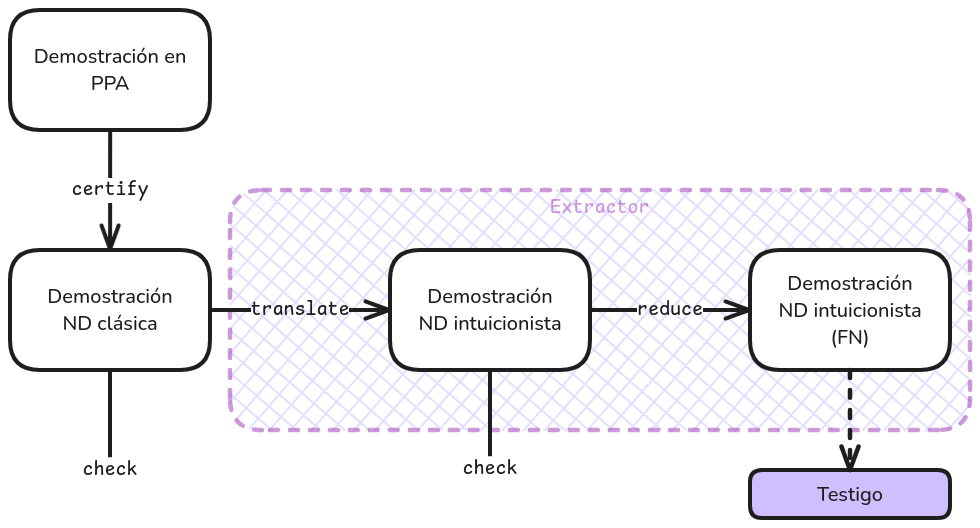
\includegraphics[width=1\linewidth]{arch.png}
\end{figure}
\end{frame}

\begin{frame}{Lógica clásica / Lógica intuicionista}
    \begin{itemize}
        \item La lógica \textbf{clásica} no siempre es constructiva, por el \textit{principio del tercero excluido} (LEM): 
        
            \begin{center}
                para toda proposición $A$, es verdadera ella o su negación
            \end{center}
        $$A \vee \neg A$$

        \item La lógica \textbf{intuicionista} se puede describir de forma sucinta como la lógica clásica sin LEM. Equivalentemente, tampoco vale la \textit{eliminación de la doble negación} ($\neg\neg A \rightarrow A$)
    \end{itemize}
\end{frame}

\begin{frame}{Demostración no constructiva}
    \begin{block}{Teorema}
        Existen dos números irracionales $a, b$ tq $a^b$ es racional.
    \end{block}
    
    Sabemos que $\sqrt{2}$ es irracional, y por LEM que $\sqrt{2}^{\sqrt{2}}$ es o racional o irracional.
    \begin{itemize}
        \item Si $\sqrt{2}^{\sqrt{2}}$ es racional, tomamos $a = b = \sqrt{2}$
        \item Sino, tomamos $a = \sqrt{2}^{\sqrt{2}}$, $b = \sqrt{2}$ y luego
        \[a^b
            = (\sqrt{2}^{\sqrt{2}})^{\sqrt{2}}
            = \sqrt{2}^{\sqrt{2} \sqrt{2}}
            = \sqrt{2}^2 = 2
        \]
        que es racional.
    \end{itemize}

    \vspace{1cm}
    \textbf{¡No nos dice cuales son $a$ y $b$!}
\end{frame}


\begin{frame}{Traducción de Friedman}

\begin{itemize}
    \item Queremos ``reducir'' o ``ejecutar'' los programas para obtener testigos de existenciales.
    \item La lógica clásica no es ejecutable (no constructiva). La intuicionista sí
    \item Friedman traduce de clásica a intuicionista. Caveat: solo fórmulas $\in \Pi^0_2$ (i.e de la forma $\forall x_1 \dots \forall x_n \exists y . \varphi)$
\end{itemize}
    
\end{frame}


% \begin{frame}{Demostración de ejemplo}
%     \begin{enumerate}
%         \item Todas las personas tienen padre. 
        
%         $$\forall H \exists P . padre(H, P)$$ 

%         \item Definición de abuelo: El padre de mi padre es mi abuelo
%         \[\forall H \forall P \forall Q
%             (padre(H, P) \wedge padre(P, Q))
%             \Rightarrow
%             abuelo(H, Q)
%         \]
%     \end{enumerate}

%     \textbf{Teorema} (Todos tienen abuelo). $\forall A \exists C . abuelo(A, C)$
    

% \begin{columns}
%     \column{0.6\textwidth}
%     \textit{Demostración}
%     \begin{itemize}
%         \item Sea $A$ una persona cualquiera.
%         \item Por (1), existe $B$, padre de $A$.
%         \item Por (1), existe $C$, padre de $B$.
%         \item Luego, por (2), $C$ es abuelo de $A$
%     \end{itemize}
%     \qed

%     \column{0.4\textwidth}
%     \begin{figure}
%         \centering
%         \includegraphics[width=0.65\linewidth]{ejemplo.png}
%     \end{figure}
% \end{columns}
% \end{frame}

% \begin{frame}[fragile]{Programa de ejemplo}
% \begin{verbatim}
% axiom todos_tienen_padre: forall P. exists Q. padre(P, Q)
% axiom def_abuelo: forall P. forall Q. forall R.
%     (padre(P, Q) & padre(Q, R)) -> abuelo(P, R)

% theorem todos_tienen_abuelo:
%     forall A. exists C. abuelo(A, C)
% proof
%     let A
%     consider B st a_padre_b: padre(A, B)
%         by todos_tienen_padre
%     consider C st b_padre_c: padre(B, C)
%         by todos_tienen_padre
    
%     take C
    
%     thus abuelo(A, C)
%         by a_padre_b, b_padre_c, def_abuelo
% end
% \end{verbatim}
% \end{frame}

\begin{frame}{¿En dónde estamos parados?}
\begin{figure}
    \centering
    %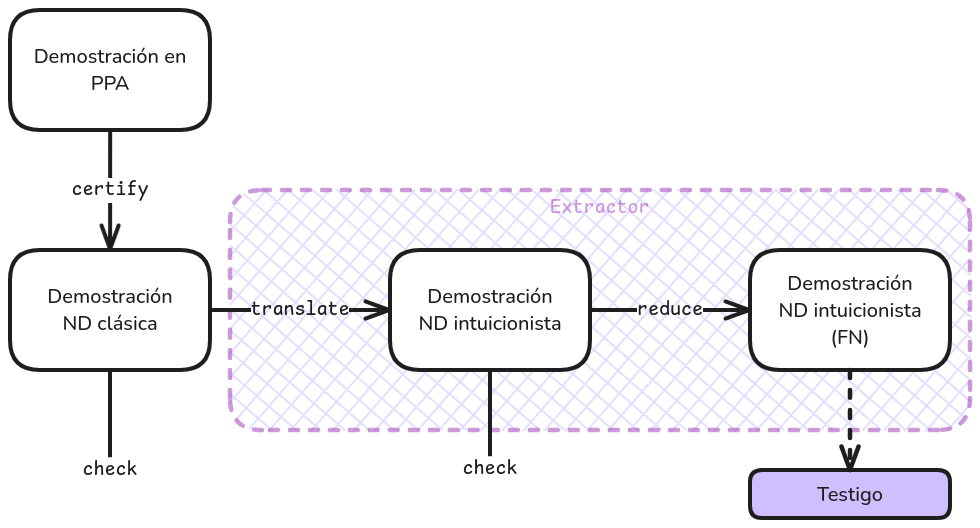
\includegraphics[width=1\linewidth]{arch.png}
\end{figure}
\end{frame}

\end{document}